\appendix

\sect{Tree Structure}

\subsect{Flattening}

A tree can be flattened for root-first traversal based on either breadth-first
search (BFS) or depth first search (DFS).

\begin{itemize}
	\item $i$ is the zero-indexed traversal order, corresponding to an array
	index of the flattened tree.
	\item $m$ is the branching factor of the tree.
	\item $h$ is the height of the tree.
	\item $r$ is the ``row'' where a given node resides in the tree;
	the number of tree levels removed from the root.
	\item $c$ is the ``column'' where a given node resides  in the tree;
	the number of nodes away from the left edge.
\end{itemize}


\begin{figure}[H]
	\centering
	\begin{tikzpicture}[
			xscale=0.7,
			tree/.style={draw,circle,inner sep=0.25mm, minimum size=14pt}
		]
		\node[tree] at (0, 0) (00) {$0,0$};
		\foreach \r [
			evaluate = \r as \w using int(3^\r),
			evaluate = \r as \wl using int(3^\r-1)
		] in {1,...,2} {
			% Columns
			\foreach \c [
				evaluate = \c as \i using int((\w-1)/2 + \c),
				evaluate = \c as \pr using int(\r-1),
				evaluate = \c as \pc using int(\c/3),
			] in {0,...,\wl} {
				\node[tree] (\r\c)
					at (\c, -\r) {$\r,\c$};
				\draw[-] (\pr\pc.south)
					-- ++(0, {-((3-\pc) + (\pr-1))/9}) -| (\r\c);
			}
		}
		\node[anchor=east] (legend) at (00 -| 28) {Node text is $r,c$};
		\node[anchor=east, below=0.1 of legend] {$m=3, h=3$};
	\end{tikzpicture}
\end{figure}


\subsubsect{BFS}

$$
	i = c + \sum_{k=1}^r m^k
	= c + \frac{1 - m^r}{1 - m}
$$

\tikzmath{\treem = 3; \treeh = 3;}

\begin{figure}[H]
	\centering
	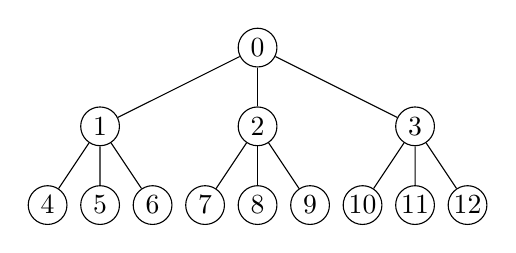
\begin{tikzpicture}[
			xscale=1.2,
			tree/.style={draw,circle,inner sep=0.25mm, minimum size=14pt}
		]
		\node[tree] at (0, 0) (00) {0};
		\foreach \r [
			evaluate = \r as \w using int(3^\r),
			evaluate = \r as \wl using int(3^\r-1)
		] in {1,...,2} {
			% Columns
			\foreach \c [
				evaluate = \c as \i using int((\w-1)/2 + \c),
				evaluate = \c as \pr using int(\r-1),
				evaluate = \c as \pc using int(\c/3),
			] in {0,...,\wl} {
				\node[tree] (\r\c)
					at ({(\c-int(\w/2)) / (\w/5)}, -\r) {\i};
				\draw[-] (\pr\pc) -- (\r\c);
			}
		}
	\end{tikzpicture}
\end{figure}

A level $k$ down the tree from the root will contain $m^k$ nodes.
Thus, a tree of with $h$ levels will contain
$\sum_{k=1}^h m^k = \frac{1-m^h}{1-m}$ nodes.

The ratio of leaf nodes to internal nodes is given by:
$$
	\frac{m^{h-1}}{\pfrac{1-m^{h-1}}{1-m}}
	= \frac{m^{h-1}(1-m)}{1-m^{h-1}}
	= \frac{m^{h-1}-m^{h}}{1-m^{h-1}}
	% = \frac{m^h-m^{h+1}}{m-m^h}
	% = \frac{m^h(1-m)}{m^h(m^{1-h} - 1)}
	= \frac{1-m}{m^{1-h} - 1}
$$

\subsubsect{DFS}

$$
	i = r + c\sum_{k=1}^{h-r} m^k
		+ \sum_{k=1}^{h-2} \left\lfloor\frac{c}{m^k}\right\rfloor
	= r + c\pfrac{1 - m^{h-r}}{1 - m}
		+ \sum_{k=1}^{h-2} \left\lfloor\frac{c}{m^k}\right\rfloor
$$

\begin{figure}[H]
	\centering
	\begin{tikzpicture}[
			xscale=1.2,
			tree/.style={draw,circle,inner sep=0.25mm, minimum size=14pt}
		]
		\node[tree] at (0, 0) (00) {0};
		\foreach \r [
			evaluate = \r as \w using int(3^\r),
			evaluate = \r as \wl using int(3^\r-1)
		] in {1,...,2} {
			% Columns
			\foreach \c [
				evaluate = \c as \i using int(
					\r + \c*(
						1 - (\treem^(\treeh-\r))
					)/(
						1 - \treem
					) + int(\c/3) + int(\c/9)
				),
				evaluate = \c as \pr using int(\r-1),
				evaluate = \c as \pc using int(\c/3),
			] in {0,...,\wl} {
				\node[tree] (\r\c)
					at ({(\c-int(\w/2)) / (\w/5)}, -\r) {\i};
				\draw[-] (\pr\pc) -- (\r\c);
			}
		}
	\end{tikzpicture}
\end{figure}
